\documentclass[tikz,border=6pt]{standalone}
\usepackage[T1]{fontenc}
\usepackage{lmodern}
\usepackage{pgfplots}
\pgfplotsset{compat=1.18}
\usetikzlibrary{arrows.meta,positioning}

\definecolor{orblue}{RGB}{76,120,168}
\definecolor{ororange}{RGB}{209,143,0}
\definecolor{orgreen}{RGB}{80,140,90}
\definecolor{orred}{RGB}{190,60,60}
% Generated by scripts/hybrid_rule.py -- do not hand-edit.
\def\HybridTheoryRows{3 & 0.30 & 0.6 & 36.3 & 36.5 & 41.0 \\
3 & 0.30 & 0.8 & 36.3 & 50.4 & 52.2 \\
3 & 0.60 & 0.6 & 74.4 & 67.1 & 77.5 \\
3 & 0.60 & 0.8 & 74.4 & 80.7 & 84.8 \\
3 & 0.85 & 0.6 & 95.8 & 88.6 & 96.4 \\
3 & 0.85 & 0.8 & 95.8 & 94.9 & 97.9 \\
6 & 0.30 & 0.6 & 63.0 & 43.6 & 66.7 \\
6 & 0.30 & 0.8 & 63.0 & 70.7 & 77.1 \\
6 & 0.60 & 0.6 & 96.5 & 73.9 & 97.0 \\
6 & 0.60 & 0.8 & 96.5 & 93.3 & 98.2 \\
6 & 0.85 & 0.6 & 100.0 & 91.7 & 100.0 \\
6 & 0.85 & 0.8 & 100.0 & 98.8 & 100.0 \\}
\def\HybHomN{164}
\def\HybHomTies{11}
\def\HybHomOpp{6}
\def\HybHomSC{84.1}
\def\HybHomCop{83.5}
\def\HybHomHyb{84.1}
\def\HybHomBSC{1}
\def\HybHomCSC{1}
\def\HybHomBCop{4}
\def\HybHomCCop{3}
\def\HybHomPSC{1.000}
\def\HybHomPCop{1.000}
\def\HybHetN{200}
\def\HybHetTies{11}
\def\HybHetOpp{8}
\def\HybHetSC{92.5}
\def\HybHetCop{85.5}
\def\HybHetHyb{92.0}
\def\HybHetBSC{1}
\def\HybHetCSC{2}
\def\HybHetBCop{14}
\def\HybHetCCop{1}
\def\HybHetPSC{1.000}
\def\HybHetPCop{$<$0.001}
\def\HybridAuditRows{Hom. AIME 2025 & 30 & 4/2 & 83.3 & 90.0 & 83.3 & 1/1 (1.000) & 0/2 (0.500) \\
Hom. AIME 2026 & 9 & 1/0 & 66.7 & 66.7 & 66.7 & 0/0 (--) & 0/0 (--) \\
Hom. MATH L5 & 25 & 1/0 & 84.0 & 84.0 & 84.0 & 0/0 (--) & 0/0 (--) \\
Hom. MMLU-Pro & 100 & 5/4 & 86.0 & 83.0 & 86.0 & 0/0 (--) & 4/1 (0.375) \\
Hom. All & 164 & 11/6 & 84.1 & 83.5 & 84.1 & 1/1 (1.000) & 4/3 (1.000) \\
Het. AIME 2026 & 29 & 1/1 & 93.1 & 82.8 & 96.6 & 1/0 (1.000) & 4/0 (0.125) \\
Het. GSM8K & 38 & 1/1 & 100.0 & 100.0 & 100.0 & 0/0 (--) & 0/0 (--) \\
Het. MATH L5 & 133 & 9/6 & 90.2 & 82.0 & 88.7 & 0/2 (0.500) & 10/1 (0.012) \\
Het. All & 200 & 11/8 & 92.5 & 85.5 & 92.0 & 1/2 (1.000) & 14/1 ($<$0.001) \\}

% generated by scripts/collision_model.py
\def\CollHomN{164}
\def\CollHomP{0.83}
\def\CollHomS{0.52}
\def\CollHomQ{0.55}
\def\CollHomPl{84.1}
\def\CollHomGone{83.5}
\def\CollHomGinf{83.5}
\def\CollHomB{4}
\def\CollHomC{5}
\def\CollHomPV{1.00}
\def\CollHomNeedInf{0.91}
\def\CollHomNeedOne{0.91}
\def\CollHetN{200}
\def\CollHetP{0.84}
\def\CollHetS{0.38}
\def\CollHetQ{0.59}
\def\CollHetPl{92.5}
\def\CollHetGone{91.0}
\def\CollHetGinf{86.0}
\def\CollHetB{0}
\def\CollHetC{3}
\def\CollHetPV{0.25}
\def\CollHetNeedInf{0.99}
\def\CollHetNeedOne{0.84}
\newcommand{\CollN}{5}\newcommand{\CollQ}{0.8}
\newcommand{\CollRows}{%
0.3 & 0.0 & 54.4 & 58.7 (0.53) & 52.5 (0.84) & 49.3 (1.00) \\
0.3 & 0.5 & 39.8 & 44.6 (0.26) & 47.5 (0.67) & 50.4 (0.99) \\
0.3 & 0.9 & 20.9 & 23.2 (0.08) & 39.4 (0.44) & 61.4 (0.90) \\
0.5 & 0.0 & 84.4 & 86.2 (0.19) & 80.0 (0.50) & 70.6 (0.97) \\
0.5 & 0.5 & 72.5 & 76.6 (0.17) & 76.6 (0.51) & 71.1 (0.97) \\
0.5 & 0.9 & 54.7 & 57.0 (0.08) & 70.2 (0.57) & 75.9 (0.95) \\
0.7 & 0.0 & 97.5 & 97.8 (0.03) & 95.2 (0.16) & 81.8 (0.83) \\
0.7 & 0.5 & 93.0 & 94.6 (0.06) & 93.3 (0.23) & 81.9 (0.83) \\
0.7 & 0.9 & 85.7 & 86.6 (0.03) & 89.3 (0.38) & 82.8 (0.83) \\}
\newcommand{\CollBERows}{%
0.3 & 0.88 & 0.63 & 0.50 \\
0.5 & 0.96 & 0.82 & 0.57 \\
0.7 & 0.99 & 0.94 & 0.84 \\}


\begin{document}
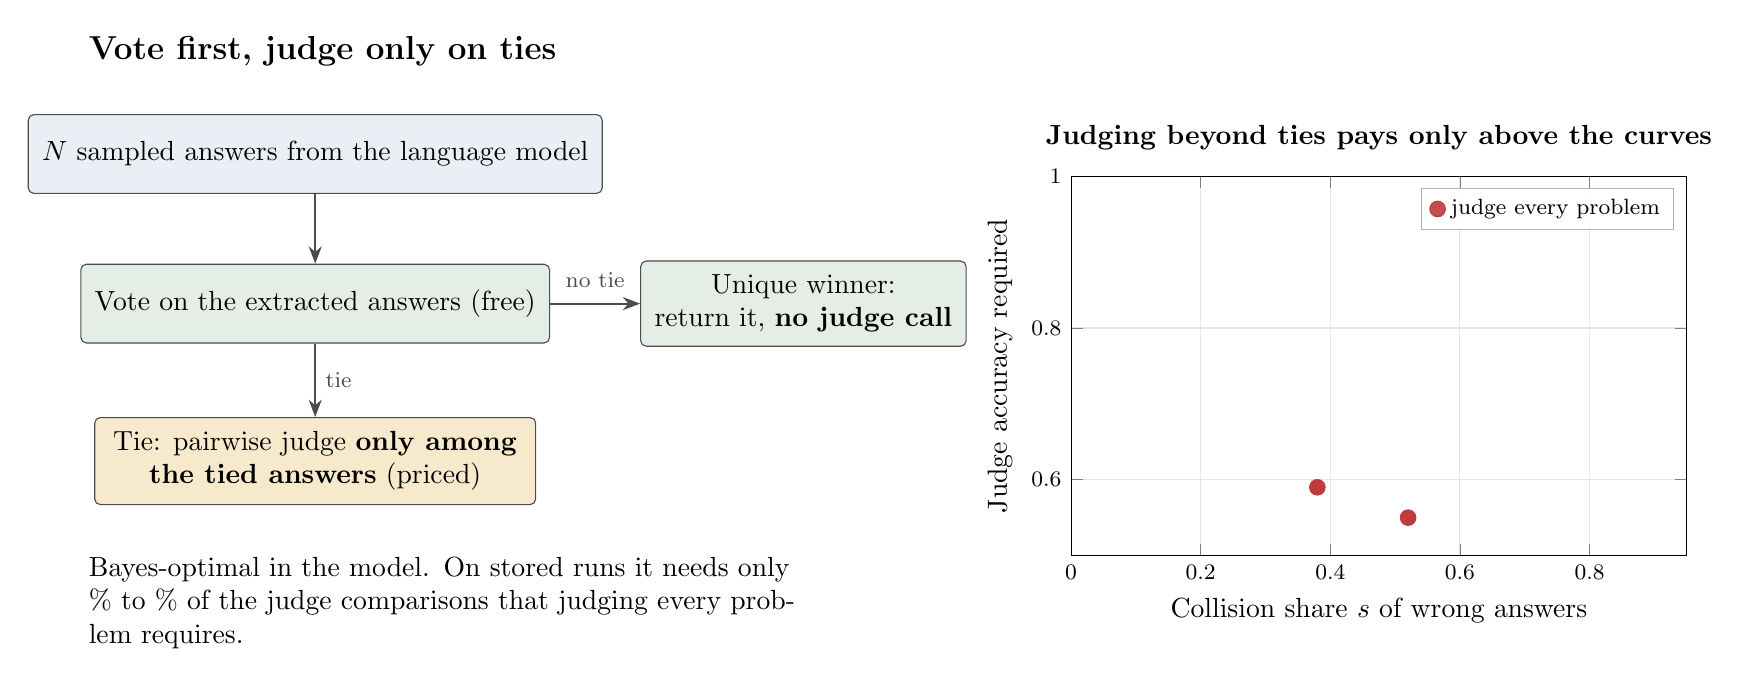
\begin{tikzpicture}[
  box/.style={draw=black!70,rounded corners=2pt,align=center,font=\normalsize,minimum height=1.0cm,inner sep=5pt,fill=white},
  arr/.style={-{Stealth[length=2.2mm]},thick,black!70}
]
% ---- left: the decision rule
\node[font=\bfseries\large,anchor=west] at (0,6.6) {Vote first, judge only on ties};
\node[box,fill=orblue!12,minimum width=5.6cm] (cand) at (3.0,5.3) {$N$ sampled answers from the language model};
\node[box,fill=orgreen!15,minimum width=5.6cm] (vote) at (3.0,3.4) {Vote on the extracted answers (free)};
\node[box,fill=orgreen!15,minimum width=3.6cm] (ret) at (9.2,3.4) {Unique winner:\\return it, \textbf{no judge call}};
\node[box,fill=ororange!20,minimum width=5.6cm] (judge) at (3.0,1.4) {Tie: pairwise judge \textbf{only among}\\\textbf{the tied answers} (priced)};
\draw[arr] (cand) -- (vote);
\draw[arr] (vote) -- node[above,font=\footnotesize,above=2pt]{no tie} (ret);
\draw[arr] (vote) -- node[right,font=\footnotesize]{tie} (judge);
\node[font=\normalsize,text width=9.0cm,align=left,anchor=north west] at (0,0.3)
  {Bayes-optimal in the model. On stored runs it needs only \HybHetCallShare\% to \HybHomCallShare\% of the judge comparisons that judging every problem requires.};

% ---- right: when judging beyond ties pays
\begin{axis}[
  at={(12.6cm,0.2cm)},anchor=south west,
  width=9.4cm,height=6.4cm,
  xmin=0,xmax=0.95,ymin=0.5,ymax=1.0,
  xlabel={Collision share $s$ of wrong answers},
  ylabel={Judge accuracy required},
  title={\bfseries Judging beyond ties pays only above the curves},
  title style={font=\normalsize},
  label style={font=\normalsize},tick label style={font=\footnotesize},
  legend style={font=\footnotesize,at={(0.98,0.97)},anchor=north east,draw=black!30,fill=white,fill opacity=0.9,text opacity=1},
  grid=both,grid style={black!10},
]
\addplot[thick,orblue] coordinates {\CollCurveInf};
\addlegendentry{judge every problem}
\addplot[thick,ororange,dashed] coordinates {\CollCurveOne};
\addlegendentry{judge when vote margin $\le 1$}
\addplot[only marks,mark=*,mark size=2.8pt,orred] coordinates {(\CollHomS,\CollHomQ) (\CollHetS,\CollHetQ)};
\addlegendentry{tested judge (measured)}
\end{axis}
\end{tikzpicture}
\end{document}
